\begin{figure}[htbp]
    \captionsetup[subfigure]{justification=centering}
    \centering
    \begin{subfigure}[b]{0.3\textwidth}
        \centering
        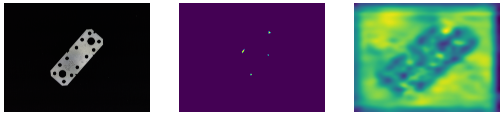
\includegraphics[width=\textwidth]{figures/ensembleimagesFC/image_prediction_100.png}
        %\caption*{Logical Anomalies}

    \end{subfigure}
    \begin{subfigure}[b]{0.3\textwidth}
        \centering
        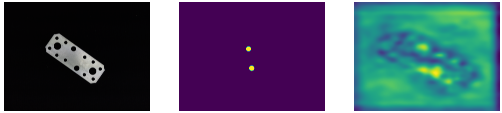
\includegraphics[width=\textwidth]{figures/ensembleimagesFC/image_prediction_036.png}


    \end{subfigure}
    \begin{subfigure}[b]{0.3\textwidth}
        \centering
        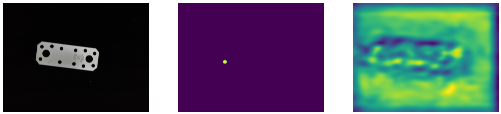
\includegraphics[width=\textwidth]{figures/ensembleimagesFC/image_prediction_052.png}


    \end{subfigure}
    \begin{subfigure}[b]{0.3\textwidth}
        \centering
        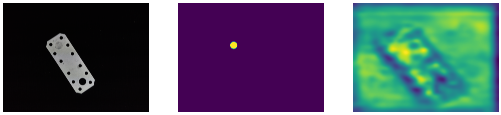
\includegraphics[width=\textwidth]{figures/ensembleimagesFC/image_prediction_061.png}
        %\caption*{Structural Anomalies}

    \end{subfigure}
    \begin{subfigure}[b]{0.3\textwidth}
        \centering
        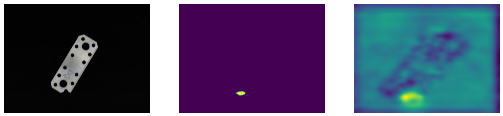
\includegraphics[width=\textwidth]{figures/ensembleimagesFC/image_prediction_073.png}


    \end{subfigure}
    \begin{subfigure}[b]{0.3\textwidth}
        \centering
        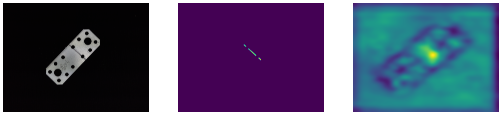
\includegraphics[width=\textwidth]{figures/ensembleimagesFC/image_prediction_085.png}


    \end{subfigure}
    \caption{Representative segmentation results from our stacking ensemble with different Wideresnet50 backbones at the same hierarchy level. The predictions are done on the novel flat 
             connector class.}
    \label{fig:ensembleFCimages}
\end{figure}